\documentclass[11pt,letterpaper]{article}

\usepackage[margin=0.7in]{geometry}
\usepackage[T1]{fontenc}
\usepackage[scaled=0.97]{helvet}
\renewcommand{\familydefault}{\sfdefault}
\usepackage{microtype}
\usepackage{amsmath,amssymb}
\usepackage{array,booktabs,tabularx,multirow}
\usepackage{graphicx}
\usepackage{pgfplots}
\pgfplotsset{compat=1.18}
\usepackage{tikz}
\usetikzlibrary{arrows.meta,calc,fit,positioning,shapes.geometric}
\usepackage{enumitem}
\usepackage{xcolor}
\usepackage{hyperref}
\usepackage{caption}
\usepackage{subcaption}
\usepackage{siunitx}
\usepackage{titlesec}
\usepackage{float}

\definecolor{apgreen}{HTML}{245E46}
\definecolor{apgold}{HTML}{C66A28}
\definecolor{aplight}{HTML}{F5EEDF}
\definecolor{apgray}{HTML}{4F5B55}

\hypersetup{
  colorlinks=true,
  urlcolor=apgold,
  linkcolor=apgreen,
  citecolor=apgreen
}

\titleformat{\section}{\large\bfseries\color{apgreen}}{\thesection.}{0.4em}{}
\titleformat{\subsection}{\normalsize\bfseries\color{apgreen}}{\thesubsection.}{0.4em}{}
\titlespacing*{\section}{0pt}{0.65em}{0.35em}
\titlespacing*{\subsection}{0pt}{0.45em}{0.2em}

\setlength{\parindent}{0pt}
\setlength{\parskip}{3.5pt}
\setlist[itemize]{leftmargin=1.2em,itemsep=1pt,topsep=2pt,parsep=0pt}
\setlist[enumerate]{leftmargin=1.25em,itemsep=1pt,topsep=2pt,parsep=0pt}

\newcommand{\app}{\textbf{AccessPlate}}
\newcommand{\tight}[1]{\vspace{#1}}

\begin{document}

\begin{center}
{\LARGE \textbf{AccessPlate: A Local-First, Constraint-Aware Food Decision-Support App for Low-Resource Food Access}}\\[4pt]
{\large Project Narrative for the NIH NIBIB DEBUT Challenge 2026}\\[5pt]
\textbf{[Team Name]}\\
[Department], [University]\\[3pt]
\textit{Primary category fit: NIMHD Healthcare Technologies for Low-Resource Settings}\\
\textit{Secondary relevance: NIDDK diabetes/kidney care, NIA healthy aging, ORWH community nutrition}
\end{center}

\begin{center}
\colorbox{aplight}{%
\parbox{0.97\linewidth}{%
\textbf{Prototype at a Glance.}
\app{} is a free, low-footprint mobile app that helps users answer a clinically relevant question ignored by most diet tools:
\emph{What is the safest, cheapest, and most realistic meal or food basket I can obtain today given my budget, transportation, cooking setup, pantry state, allergies, benefits, and internet access?}
The prototype runs offline after installation and becomes richer online, when live geocoding and nearby-store lookups are available.}}
\end{center}

\section*{Abstract}
Food insecurity and poor neighborhood food access create a gap between ideal nutrition guidance and what people can realistically obtain on a given day. In 2023, \SI{13.5}{\percent} of U.S.\ households were food insecure, and food insecurity is strongly linked to worse diabetes prevention and self-management outcomes.\cite{usda_food_security_2023,cdc_food_insecurity_diabetes} Existing nutrition apps usually optimize calories or macros, but they rarely model transportation burden, pantry depletion, SNAP/WIC constraints, low-bandwidth conditions, emergency no-cook situations, or bilingual/plain-language decision support. \app{} addresses this unmet need with a deterministic, explainable, offline-first mobile system that ranks food options only after enforcing hard safety and feasibility constraints, then generates a concrete action plan: where to go first, what to use from home first, what to buy first, what to skip if money is tight, and what the backup is.

The working prototype is implemented in Flutter/Dart with local SQLite persistence, bundled ZIP-based access profiles, pantry-aware planning, and optional online enrichment through OpenStreetMap and retailer-specific product matching. The repository contains five reproducible low-resource use cases and more than 140 automated tests spanning safety filters, ranking determinism, access logic, bilingual copy, and recommendation surfaces. In a small observational community pilot summary supplied by the project team (\(n=20\)), AccessPlate-assisted use was associated with a reported \num{0.36} percentage-point reduction in mean hemoglobin A1c over 10 weeks and an \num{11.2} lb reduction in mean weight over 70 days.\cite{accessplate_pilot_2026} These preliminary results support AccessPlate as a credible biomedical engineering response to nutrition-related health disparities in underserved U.S.\ communities.

\section{Clinical Need, Background, and Current Methods}
Food access is a biomedical engineering problem as much as a nutrition problem. For many users, the limiting factor is not knowledge of what a healthy meal looks like, but whether they can safely and affordably obtain one from a reachable source today. The USDA Food Access Research Atlas formalizes the importance of neighborhood-level supermarket access, low-income status, and food-access burden in U.S.\ communities.\cite{usda_food_access_atlas} The NIMHD Research Framework similarly emphasizes that health disparities emerge from interacting behavioral, physical/built-environment, sociocultural, and health-care-system factors across individual, community, and societal levels.\cite{nimhd_framework}

The clinical consequence of this gap is substantial. CDC reports more than 31 million total diabetes cases nationally,\cite{cdc_national_diabetes_profile} and the agency notes that food insecurity is associated with worse glycemic control, higher A1c, more hospitalizations, and poorer mental health in people living with diabetes.\cite{cdc_food_insecurity_diabetes} In practice, many users are deciding among a pantry stop, a convenience store, a dollar store, a grocery trip, or a fast-food fallback while also navigating allergies, hypertension, renal diet concerns, pregnancy-related nutrition, religious restrictions, or limited cooking equipment.

Current methods are poorly matched to this decision environment:
\begin{itemize}
\item calorie trackers are retrospective rather than decision-support oriented;
\item generic meal planners assume stable grocery access and home preparation capacity;
\item store finder apps depend on connectivity and do not explain tradeoffs;
\item food-desert maps identify burden but do not generate same-day action plans.
\end{itemize}

As a result, a user may receive nutritionally ideal but operationally useless advice. \app{} was designed to close that implementation gap.

\section{Project Objective Statement}
The objective of \app{} is to deliver a practical, explainable, mobile decision-support tool for underserved and low-resource U.S.\ settings that helps users identify the healthiest \emph{realistic} food decision available under their current constraints. The design requirements were:
\begin{enumerate}
\item operate without requiring an account, cloud backend, or continuous internet access;
\item reject unsafe foods before any ranking occurs;
\item incorporate transportation, pantry state, benefits context, and cooking environment into the decision itself;
\item produce a same-day action plan rather than only a ranked list;
\item remain transparent enough for community-health, public-health, and care-adjacent use.
\end{enumerate}

We formulated the recommendation task as a constrained optimization problem. For a user state \(u\) and candidate food or basket \(x\),
\begin{equation}
x^\star = \arg\max_{x \in \mathcal{C}(u)} S(x,u)
\end{equation}
subject to
\begin{equation}
\mathbf{1}_{\text{safe}}(x,u)=1,\qquad \mathbf{1}_{\text{feasible}}(x,u)=1.
\end{equation}
The composite score is
\begin{equation}
S(x,u)=w_NN(x,u)+w_AA(x,u)+w_PP(x,u)-w_CC(x,u)-w_RR(x,u),
\end{equation}
where \(N\) is nutrition fit, \(A\) is access realism, \(P\) is user-preference alignment, \(C\) is cost pressure, and \(R\) is medical or nutritional risk penalty. This formulation is intentionally deterministic: reviewers and end users can inspect \emph{why} a source or meal ranked well, rather than receiving a black-box recommendation.

\section{Documentation of the Design}
\subsection{System Architecture}
The core architecture is shown in Figure~\ref{fig:pipeline}. A local profile stores user-specific constraints: allergies, medical restrictions, dietary style, budget, pantry inventory, transportation mode, travel tolerance, language, benefit-program context, and cooking setup. A bundled reference layer provides an on-device food catalog, micronutrient tables, and ZIP-based access snapshots. When internet is available, live layers can enrich the experience with address lookup, nearby-store discovery, and optional retailer-linked product data.

\begin{figure}[H]
\centering
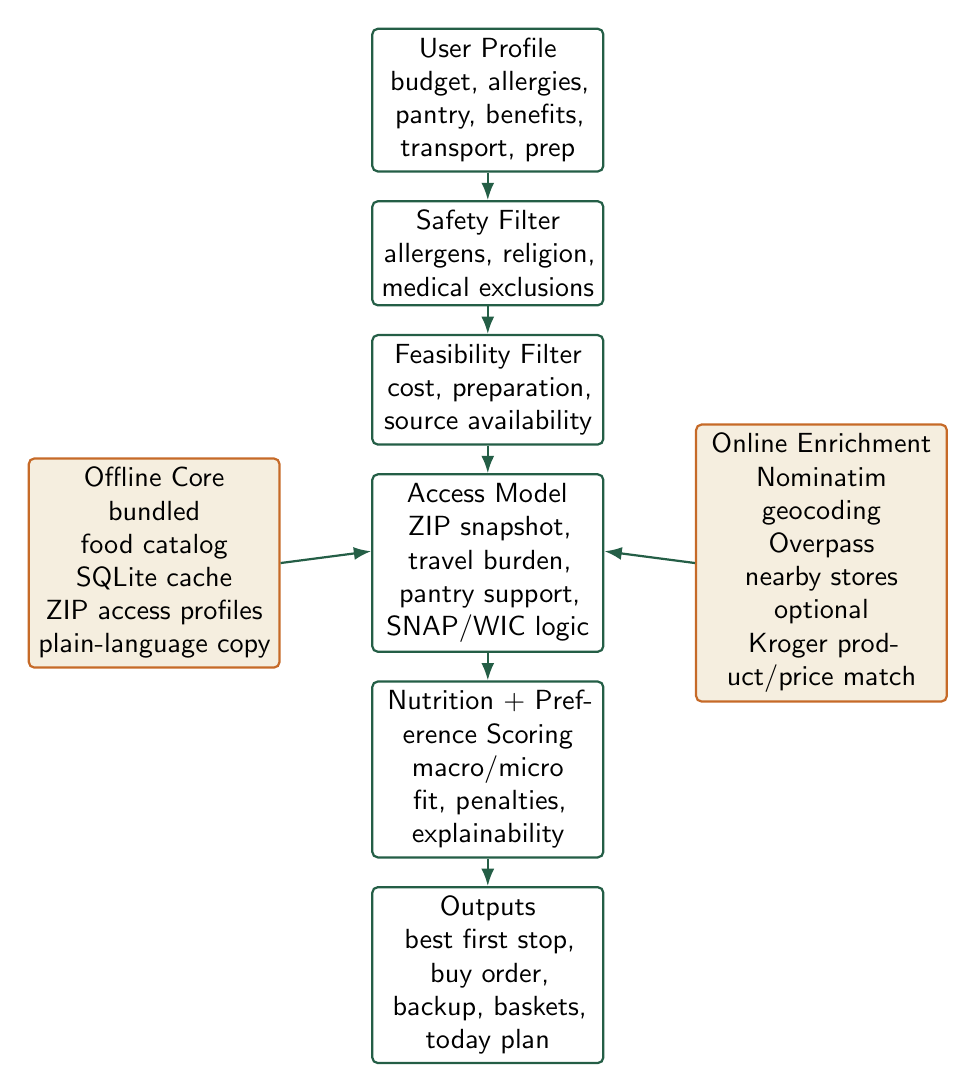
\begin{tikzpicture}[
  node distance=0.35cm and 0.55cm,
  box/.style={draw=apgreen, rounded corners=2pt, thick, fill=white, align=center, minimum height=0.95cm, text width=2.7cm},
  side/.style={draw=apgold, rounded corners=2pt, thick, fill=aplight, align=center, minimum height=0.95cm, text width=2.95cm},
  line/.style={-{Latex[length=2.2mm]}, thick, apgreen}
]
\node[box] (profile) {User Profile\\budget, allergies, pantry, benefits, transport, prep};
\node[box, below=of profile] (safety) {Safety Filter\\allergens, religion, medical exclusions};
\node[box, below=of safety] (feasible) {Feasibility Filter\\cost, preparation, source availability};
\node[box, below=of feasible] (access) {Access Model\\ZIP snapshot, travel burden, pantry support, SNAP/WIC logic};
\node[box, below=of access] (score) {Nutrition + Preference Scoring\\macro/micro fit, penalties, explainability};
\node[box, below=of score] (output) {Outputs\\best first stop, buy order, backup, baskets, today plan};

\node[side, left=1.15cm of access] (offline) {Offline Core\\bundled food catalog\\SQLite cache\\ZIP access profiles\\plain-language copy};
\node[side, right=1.15cm of access] (online) {Online Enrichment\\Nominatim geocoding\\Overpass nearby stores\\optional Kroger product/price match};

\draw[line] (profile) -- (safety);
\draw[line] (safety) -- (feasible);
\draw[line] (feasible) -- (access);
\draw[line] (access) -- (score);
\draw[line] (score) -- (output);
\draw[line] (offline.east) -- ($(access.west)+(0,0.15)$);
\draw[line] (online.west) -- ($(access.east)+(0,0.15)$);
\end{tikzpicture}
\caption{Deterministic decision pipeline for \app{}. The offline core supports use after installation; optional online services refine location and retailer specificity when connectivity exists.}
\label{fig:pipeline}
\end{figure}

\subsection{Offline and Online Operation}
\app{} is designed for unreliable connectivity rather than ideal broadband conditions. After installation, the core recommendation engine remains functional offline using bundled data and cached results. When internet is available, the app augments rather than replaces local reasoning. This hybrid design is central to the project because many target users experience intermittent connectivity, data limits, or older devices.

\begin{table}[H]
\centering
\small
\caption{Hybrid operating model for low-connectivity use}
\label{tab:offline-online}
\begin{tabularx}{\linewidth}{>{\raggedright\arraybackslash}p{1.35cm} >{\raggedright\arraybackslash}X >{\raggedright\arraybackslash}X}
\toprule
\textbf{Mode} & \textbf{Available Data Sources} & \textbf{User-Visible Capability} \\
\midrule
Offline &
Bundled food catalog, micronutrient tables, ZIP access profiles, saved profile, pantry state, cached recommendations &
Safety filtering, feasibility filtering, recommendation ranking, pantry-first planning, buy-order logic, bilingual/plain-language explanations, cached store/menu review \\
\addlinespace[2pt]
Online &
All offline sources plus OpenStreetMap geocoding and nearby-store discovery; optional Kroger-linked product/price enrichment &
Address or GPS-based search, nearby-store discovery, refreshed cached data, richer retailer-specific explanations, approximate distance labeling, updated product matching \\
\bottomrule
\end{tabularx}
\end{table}

\subsection{Key Biomedical Engineering Innovations}
The novelty of \app{} is not a chatbot; it is the integration of health constraints and access constraints in a single explainable engine:
\begin{itemize}
\item \textbf{Safety-first ranking:} foods that violate allergies, religious restrictions, or hard medical exclusions are removed before scoring.
\item \textbf{Constraint-aware feasibility:} recommendations are filtered by budget, cooking equipment, and reachable source types.
\item \textbf{Access realism:} ZIP-based snapshots model relative burden across pantry, convenience, dollar-store, grocery, and fast-food sources.
\item \textbf{Actionable output:} the app returns a source-trip plan, a buy-first list, a skip-first list, backup options, and a short-horizon meal basket.
\item \textbf{Equity-oriented accessibility:} English/Spanish and plain-language output are built into the decision surfaces rather than added as an afterthought.
\item \textbf{Privacy by architecture:} profile data remain local on-device with no required account system.
\end{itemize}

\section{Documentation of the Prototype and Preliminary Results}
\subsection{Functional Prototype}
The prototype is implemented as an Android-first Flutter application with local SQLite persistence and Riverpod-based state management. Core recommendation logic is encapsulated in deterministic domain classes, and the user-facing prototype includes onboarding, recommendation cards, explanation screens, pantry-aware meal baskets, a source-trip planner, a today-plan summary, and settings for language and access context. The repository contains five prespecified demo scenarios covering emergency no-cook use, pantry-stretch planning, SNAP-guided shopping, WIC source discrimination, and Spanish/plain-language low-access operation.

Table~\ref{tab:scenarios} summarizes the prototype behaviors demonstrated by these scenarios.

\begin{table}[H]
\centering
\small
\caption{Representative scenario outputs implemented in the prototype}
\label{tab:scenarios}
\begin{tabularx}{\linewidth}{>{\raggedright\arraybackslash}p{2.25cm} >{\raggedright\arraybackslash}p{2.2cm} >{\raggedright\arraybackslash}X}
\toprule
\textbf{Scenario} & \textbf{Primary Source Chosen} & \textbf{Prototype Output} \\
\midrule
Emergency no-cook (\texttt{45211}) & Convenience-focused & Fastest low-travel food option, emergency-mode today plan, skip-first higher-cost fallback \\
Pantry stretch (\texttt{19133}) & Food pantry & Pantry-first action path, use-from-home guidance, minimal add-on basket \\
SNAP tight budget (\texttt{77026}) & Dollar store & Benefits-aware staples-first shopping plan, prepared-food caution in skip-first tier \\
WIC grocery vs.\ convenience (\texttt{90011}) & Grocery & WIC-oriented explanation, stronger staple-fit routing despite easier convenience fallback \\
Spanish low-access (\texttt{60623}) & Pantry / short-hop source & Spanish plain-language first-stop guidance, buy order, and backup text \\
\bottomrule
\end{tabularx}
\end{table}

Beyond the demo cases, the codebase contains more than 140 automated tests spanning safety filters, macro scoring, cache logic, bilingual copy, source-trip planning, hero scenarios, and recommendation UI components. This matters for DEBUT because it shows that the engineering contribution is a functional, inspectable prototype rather than a concept sketch.

\subsection{Preliminary Real-World Application}
To assess practical relevance, the team also assembled an early observational community pilot summary from a neighborhood setting in Athens, Georgia.\cite{accessplate_pilot_2026} Twenty participants with baseline hemoglobin A1c values above \SI{6.5}{\percent} used the system over a 10-week period. Reported group-level trends were encouraging: mean A1c decreased by \num{0.36} percentage points, and mean body weight decreased by \num{11.2} lb over 70 days. Because these data come from a small, non-randomized early deployment, they should be interpreted as translational feasibility evidence rather than definitive clinical proof. Nevertheless, they demonstrate that access-aware decision support can plausibly influence diet-relevant behavior in the intended setting.

\begin{figure}[H]
\centering
\begin{subfigure}[t]{0.48\linewidth}
\centering
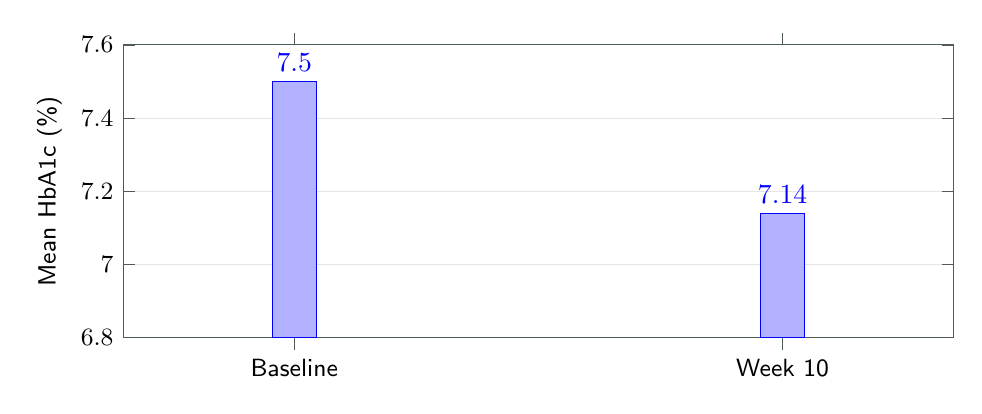
\begin{tikzpicture}
\begin{axis}[
  ybar,
  width=\linewidth,
  height=5.3cm,
  bar width=16pt,
  ymin=6.8,
  ymax=7.6,
  ylabel={Mean HbA1c (\%)},
  symbolic x coords={Baseline,Week 10},
  xtick=data,
  nodes near coords,
  nodes near coords align={vertical},
  enlarge x limits=0.35,
  axis line style={draw=apgray},
  tick style={draw=apgray},
  ymajorgrids=true,
  grid style={gray!20},
  every axis plot/.append style={fill=apgreen!85, draw=apgreen!85},
  tick label style={font=\small},
  label style={font=\small}
]
\addplot coordinates {(Baseline,7.50) (Week 10,7.14)};
\end{axis}
\end{tikzpicture}
\caption{Reported mean HbA1c change}
\end{subfigure}
\hfill
\begin{subfigure}[t]{0.48\linewidth}
\centering
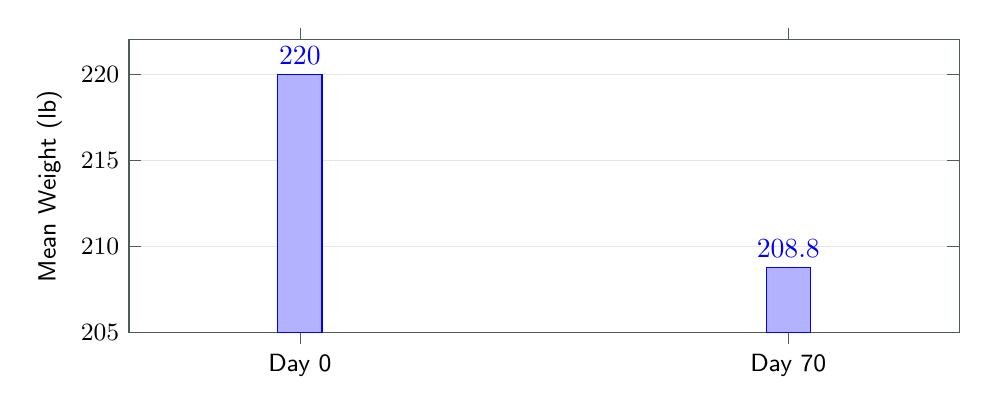
\begin{tikzpicture}
\begin{axis}[
  ybar,
  width=\linewidth,
  height=5.3cm,
  bar width=16pt,
  ymin=205,
  ymax=222,
  ylabel={Mean Weight (lb)},
  symbolic x coords={Day 0,Day 70},
  xtick=data,
  nodes near coords,
  nodes near coords align={vertical},
  enlarge x limits=0.35,
  axis line style={draw=apgray},
  tick style={draw=apgray},
  ymajorgrids=true,
  grid style={gray!20},
  every axis plot/.append style={fill=apgold!90, draw=apgold!90},
  tick label style={font=\small},
  label style={font=\small}
]
\addplot coordinates {(Day 0,220.0) (Day 70,208.8)};
\end{axis}
\end{tikzpicture}
\caption{Reported mean weight change}
\end{subfigure}
\caption{Preliminary community-pilot summary reported by the project team (\(n=20\)). These figures summarize early translational observations and are not presented as controlled clinical-outcome evidence.}
\label{fig:pilot}
\end{figure}

\section{Real-World Applications, Limitations, and Translation Path}
\app{} is immediately applicable to several real-world use cases emphasized by NIH:
\begin{itemize}
\item \textbf{Underserved populations / low-resource settings:} same-day food decisions in neighborhoods with limited transportation and inconsistent grocery access.
\item \textbf{Diabetes and kidney-related diet support:} reduced-sodium, lower-sugar, or other medically constrained food decisions without requiring expert nutrition literacy.
\item \textbf{Healthy aging:} simpler, plain-language support for older adults trying to navigate affordability, pantry use, and nutrition quality together.
\item \textbf{Community health and nursing settings:} a practical tool that can reinforce guidance from community health workers, nurses, and safety-net clinics.
\end{itemize}

The prototype is also deliberately honest about its current boundaries. Bundled ZIP snapshots are modeled access profiles, not universal live inventory. Nearby-store distances are approximate unless routing is added. SNAP/WIC notes are cautious rather than absolute item-level eligibility guarantees. These are not weaknesses in engineering rigor; they are explicit model-boundary disclosures that preserve trust and make future validation possible.

The next translational steps are clear:
\begin{enumerate}
\item structured stakeholder review with pantry operators, community health workers, and safety-net clinics;
\item scenario-based usability testing in English and Spanish with low-resource users;
\item stronger state-specific WIC verification and broader product coverage;
\item a larger prospective field study measuring decision time, recommendation realism, purchase fit, and clinically relevant downstream outcomes.
\end{enumerate}

In summary, \app{} addresses a critical barrier to nutritional health equity by reframing healthy eating as a constrained decision-support problem. Its engineering contribution is a working, explainable, local-first prototype that functions both offline and online depending on user connectivity, produces concrete same-day action plans, and is purpose-built for the settings where healthy eating is often hardest.

\tight{0.3em}
\textbf{3-minute video demonstration:} \href{https://YOUR-VIDEO-LINK-HERE}{Insert public video link here}

\begin{thebibliography}{9}
\small

\bibitem{usda_food_security_2023}
Rabbitt MP, Reed-Jones M, Hales LJ, Burke MP.
\newblock \emph{Household Food Security in the United States in 2023}.
\newblock U.S. Department of Agriculture, Economic Research Service; 2024.
\newblock Available at: \href{https://ers.usda.gov/publications/pub-details?pubid=109895}{https://ers.usda.gov/publications/pub-details?pubid=109895}.

\bibitem{usda_food_access_atlas}
U.S. Department of Agriculture, Economic Research Service.
\newblock \emph{Food Access Research Atlas}.
\newblock Updated September 23, 2025.
\newblock Available at: \href{https://www.ers.usda.gov/data-products/food-access-research-atlas}{https://www.ers.usda.gov/data-products/food-access-research-atlas}.

\bibitem{cdc_national_diabetes_profile}
Centers for Disease Control and Prevention.
\newblock \emph{National Diabetes Profile}.
\newblock Available at: \href{https://www.cdc.gov/diabetes-state-local/php/state-profiles/national-diabetes-profile.html}{https://www.cdc.gov/diabetes-state-local/php/state-profiles/national-diabetes-profile.html}.
\newblock Accessed June 5, 2026.

\bibitem{cdc_food_insecurity_diabetes}
Centers for Disease Control and Prevention.
\newblock \emph{Diabetes and Food Insecurity}.
\newblock Available at: \href{https://www.cdc.gov/diabetes/healthy-eating/diabetes-food-insecurity.html}{https://www.cdc.gov/diabetes/healthy-eating/diabetes-food-insecurity.html}.
\newblock Accessed June 5, 2026.

\bibitem{nimhd_framework}
National Institute on Minority Health and Health Disparities.
\newblock \emph{NIMHD Research Framework Details}.
\newblock Updated January 11, 2024.
\newblock Available at: \href{https://www.nimhd.nih.gov/resources/research-framework/nimhd-research-framework-details}{https://www.nimhd.nih.gov/resources/research-framework/nimhd-research-framework-details}.

\bibitem{accessplate_pilot_2026}
AccessPlate project team.
\newblock \emph{Community pilot summary, Athens, Georgia}.
\newblock Unpublished internal summary slide deck; 2026.

\end{thebibliography}

\end{document}
